\documentclass{article}
% translate with >> pdflatex -shell-escape <file>

% This file is an extract of the PGFPLOTS manual, copyright by Christian Feuersaenger.
% 
% Feel free to use it as long as you cite the pgfplots manual properly.
%
% See
%   http://pgfplots.sourceforge.net/pgfplots.pdf
% for the complete manual.
%
% Any required input files (for <plot table> or <plot file> or the table package) can be downloaded
% at
% http://www.ctan.org/tex-archive/graphics/pgf/contrib/pgfplots/doc/latex/
% and
% http://www.ctan.org/tex-archive/graphics/pgf/contrib/pgfplots/doc/latex/plotdata/

\usepackage{pgfplots}
\pgfplotsset{compat=newest}

\pagestyle{empty}

\begin{document}
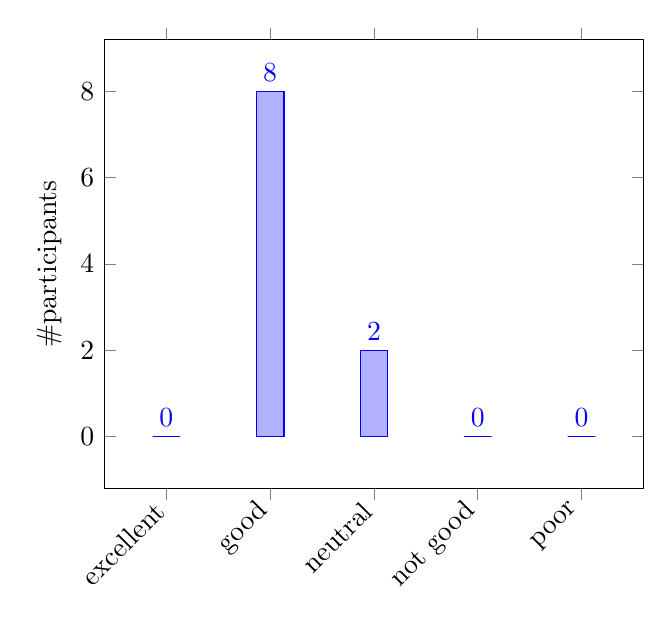
\begin{tikzpicture}
  \begin{axis}[
    ybar,
    enlargelimits=0.15,
    legend style={at={(0.5,-0.2)},
      anchor=north,legend columns=-1},
    ylabel={\#participants},
    symbolic x coords={excellent,good,neutral,%
		not good,poor},
    xtick=data,
    nodes near coords, 
	nodes near coords align={vertical},
    x tick label style={rotate=45,anchor=east},
    ]
    \addplot coordinates {(excellent,0) (good,8) 
		(neutral,2) (not good,0) (poor,0)};
  \end{axis}
\end{tikzpicture}
\end{document}
